\documentclass{report}

\usepackage[a4paper, total={6in, 8in}, margin=1in,footskip=0.25in]{geometry}
\usepackage{amsmath, amsthm, amssymb, booktabs, chemfig, gensymb, graphicx, float, pgfplots, upgreek, siunitx, multirow, multicol, setspace, longtable}
\renewcommand{\familydefault}{\sfdefault}
\usepackage[hidelinks]{hyperref}
\newcommand{\perthousand}{‰}
\newcommand{\micro}{µ}
\renewcommand{\printatom}[1]{\ensuremath{\mathrm{#1}}}
\usepackage[chemgreek=mhchem]{chemmacros}
\chemsetup[phases]{pos=sub}
\chemsetup[reactants]{concentration-unit=\moLar}
\chemsetup{
  formula = mhchem, % or mhchem
}

\DeclareSIUnit{\solub}{\unit[per-mode=symbol]{\gram\per\qty{100}{\gram}\,\ce{H2O}}}

\setlength{\parindent}{0pt}
\setlength{\parskip}{0.8em}

\pgfplotsset{compat=1.18}

\graphicspath{{../../Images/}}

\title{\Huge Year 12 Chemistry \\
	\begin{Large}
		Module 7 Depth Study
	\end{Large}}
\author{L. Cheung}

\tolerance=1
\emergencystretch=\maxdimen
\hyphenpenalty=10000
\hbadness=10000

\begin{document}
	\setstretch{1.25}

	\DeclareSIUnit{\molar}{\mole\per\liter}
	\DeclareSIUnit{\enthalpy}{\kJ\per\mole}
	\maketitle
	\newpage

\chapter*{Chapter 8 Review}

	\begin{enumerate}
		\item \textbf{Explain why carbon is the basis for so many compounds.}
			Carbon readily bonds to other carbon atoms, and has 4 valence electrons. This allows it to bond with many other elements and is therefore used as a base for compounds.

		\item \textbf{Draw electron dot diagrams to show how single, double and triple carbon-carbon bonds form.}
			\begin{center}
				\charge{0=\:, 90=\., 180=\., 270=\.}{C} \charge{0=\., 90=\., 270=\.}{C} \\
				\charge{0=\:\:,180=\:}{C} \charge{0=\:}{C} \\
				\charge{180=\., 0=\:\:\:}{C} \charge{0=\.}{C}
			\end{center}
		    
		\item \textbf{Draw diagrams and name the geometrical shapes formed when carbon atoms have:}
		\begin{enumerate}
			\item \textit{four single bonds}
				\begin{center}
					\chemfig{C(-[2])(-[6])(-[8])-[4]}
				\end{center}

				Forms a tetrahedron

			\item \textit{one double and two single bonds}
				\begin{center}
					\chemfig{C(=[0])(-[3])(-[5])}
				\end{center}

				Forms a trigonal planar

			\item \textit{two double bonds}
				\begin{center}
					\chemfig{C(=[4])(=[0])}
				\end{center}

				Forms a linear structure

			\item \textit{one triple and one single bond.}
				\begin{center}
					\chemfig{C(-[4])(~[0])}
				\end{center}

				Forms a linear structure

		\end{enumerate}
		    
		\item \textbf{Describe, with examples, the difference between saturated and unsaturated compounds.}

			Compounds are considered saturated when all carbon atoms have single bonds. For example, methane only has single bonds, hence is saturated. An unsaturated compound has at least one double or triple bonded carbon atom. An example of such is carbon dioxide.
		    
		\item \textbf{Describe, with examples, the difference between aromatic and aliphatic compounds.}

			Aliphatic compounds have open chained structures, ie. the carbon chain has a ends, for example butane. These can also be branched compounds, with alkyls attached to the main branch.

			Aromatic have one or more benzene rings, with the benzene compound being the most basic
		    
		\item \textbf{For each of the families of hydrocarbons (alkanes, alkenes and alkynes):}

			\begin{itemize}
				\item \textit{give the general formula}
				\item \textit{write the molecular and structural formula for the first five in the series; for the alkenes and alkynes, have the double and triple bond on the first carbon.}
			\end{itemize}
				
			\begin{table}[H]
				\centering
				\setstretch{1.25}
				\begin{tabular}{p{3cm}|p{3cm}|p{10cm}}
					\textbf{Alkanes} (\ce{C_{n}H_{2n+2}})	& \textbf{Molecular Formula}	& \textbf{Structural Formula}			\\ \hline
										&				&						\\
										& \ce{CH4}			& \chemfig{C(-[2]H)(-[4]H)(-[6]H)(-[8]H)}	\\
										&				&						\\
										& \ce{C2H6}			& \chemfig{C(-[2]H)(-[4]H)(-[6]H) - C(-[2]H)(-[0]H)(-[6]H)}
										&				&						\\
										& \ce{C3H8}			& \chemfig{C(-[2]H)(-[4]H)(-[6]H)-C(-[2]H)(-[6]H)-C(-[2]H)(-[6]H)(-[0]H)}	\\
										&				&						\\
										& \ce{C4H10}			& \chemfig{C(-[2]H)(-[4]H)(-[6]H)-C(-[2]H)(-[6]H)-C(-[2]H)(-[6]H)-C(-[2]H)(-[6]H)(-[0]H)}	\\
										&				&						\\
										& \ce{C5H12}			& \chemfig{C(-[2]H)(-[4]H)(-[6]H)-C(-[2]H)(-[6]H)-C(-[2]H)(-[6]H)-C(-[2]H)(-[6]H)-C(-[2]H)(-[6]H)(-[0]H)}	\\
				\end{tabular}
			\end{table}

			\begin{table}[H]
				\centering
				\setstretch{1.25}
				\begin{tabular}{p{3cm}|p{3cm}|p{10cm}}
					\textbf{Alkenes} (\ce{C_{n}H_{2n}})	& \textbf{Molecular Formula}	& \textbf{Structural Formula}			\\ \hline
										&				&						\\
										& \ce{C2H4}			& \chemfig{C(-[3]H)(-[5]H) = C(-[1]H)(-[7]H)}	\\
										&				&						\\
										& \ce{C3H6}			& \chemfig{C(-[3]H)(-[5]H) = C(-[2]H) - C(-[2]H)(-[6]H)(-[0]H)} \\
										&				&						\\
										& \ce{C4H8}			& \chemfig{C(-[3]H)(-[5]H) = C(-[2]H) - C(-[2]H)(-[6]H) - C(-[2]H)(-[6]H)(-[8]H)} \\
										&				&						\\
										& \ce{C5H10}			& \chemfig{C(-[3]H)(-[5]H) = C(-[2]H) - C(-[2]H)(-[6]H) - C(-[2]H)(-[6]H) - C(-[2]H)(-[6]H)(-[0]H)} \\
										&				&						\\
										& \ce{C6H12}			& \chemfig{C(-[3]H)(-[5]H) = C(-[2]H) - C(-[2]H)(-[6]H) - C(-[2]H)(-[6]H) - C(-[2]H)(-[6]H) - C(-[2]H)(-[6]H)(-[8]H)} \\
				\end{tabular}
			\end{table}

			\begin{table}[H]
				\centering
				\setstretch{1.25}
				\begin{tabular}{p{3cm}|p{3cm}|p{10cm}}
					\textbf{Alkynes} (\ce{C_{n}H_{2n-2}})	& \textbf{Molecular Formula}	& \textbf{Structural Formula}			\\ \hline
										&				&						\\
										& \ce{C2H2}			& \chemfig{C(-[4]H) ~ C(-[0]H)}			\\
										&				&						\\
										& \ce{C3H4}			& \chemfig{C(-[4]H) ~ C - C(-[2]H)(-[6]H)(-[0]H)} \\
										&				&						\\
										& \ce{C4H6}			& \chemfig{C(-[4]H) ~ C - C(-[2]H)(-[6]H) - C(-[2]H)(-[6]H)(-[0]H)} \\
										&				&						\\
										& \ce{C5H8}			& \chemfig{C(-[4]H) ~ C - C(-[2]H)(-[6]H) - C(-[2]H)(-[6]H) - C(-[2]H)(-[6]H)(-[8]H)} \\
										&				&						\\
										& \ce{C6H10}			& \chemfig{C(-[4]H) ~ C - C(-[2]H)(-[6]H) - C(-[2]H)(-[6]H) - C(-[2]H)(-[6]H) - C(-[2]H)(-[6]H)(-[8]H)} \\
				\end{tabular}
			\end{table}
		    
		\item \textbf{Name the following hydrocarbons.}
			\begin{enumerate}
				\item 2-methylbutane
				\item 4-ethyl-2,3,3-trimethylpropane
				\item pent-2-ene
				\item 2,4,4-trimethylpent-2-ene
				\item 3,5-dimethylhex-1-yne
				\item 4-methylhept-2-yne
				\item 1,2-dichloro-3,3-difluoropentane
				\item 1,1,4-trichloro-1,2,4-trifluorohept-2-ene
			\end{enumerate}

		\item \textbf{Draw structural formula for the following molecules.}
			\begin{enumerate}
				\item 1,1-dichloroethane
					\subitem \chemfig{C(-[2]Cl)(-[4]H)(-[6]Cl) - C(-[2]H)(-[6]H)(-[0]H)} \\

				\item 2,3-dimethylhexane
					\subitem \chemfig{C(-[2,0.6]H)(-[4,0.6]H)(-[6,0.6]H) - C(-[2]C(-[0,0.6]H)(-[2,0.6]H)(-[4,0.6]H))(-[6,0.6]H) - C(-[6]C(-[0,0.6]H)(-[6,0.6]H)(-[4,0.6]H))(-[2,0.6]H) - C(-[2,0.6]H)(-[6,0.6]H) - C(-[2,0.6]H)(-[6,0.6]H) - C(-[2,0.6]H)(-[6,0.6]H)(-[0,0.6]H)} \\

				\item 2,2,6-trimethyl-3-octene
					\subitem \chemfig{C(-[2,0.6]H)(-[4,0.6]H)(-[6,0.6]H) - C(-[2] C(-[0,0.6]H)(-[2,0.6]H)(-[4,0.6]H))(-[6] C(-[0,0.6]H)(-[6,0.6]H)(-[4,0.6]H)) - C(-[2,0.6]H) = C(-[2,0.6]H) - C(-[2,0.6]H)(-[6,0.6]H) - C(-[2]C(-[0,0.6]H)(-[2,0.6]H)(-[4,0.6]H))(-[6,0.6]H) - C(-[2,0.6]H)(-[6,0.6]H) - C(-[0,0.6]H)(-[2,0.6]H)(-[6,0.6]H)} \\

				\item 2,3-dimethyl-3-ethyl-1-pentene
					\subitem \chemfig{C(-[3,0.6]H)(-[5,0.6]H) = C(-[2]C(-[0,0.6]H)(-[2,0.6]H)(-[4,0.6]H)) - C(-[2]C(-[0,0.6]H)(-[2,0.6]H)(-[4,0.6]H))(-[6]C(-[4,0.6]H)(-[0,0.6]H)(-[6]C(-[4,0.6]H)(-[6,0.6]H)(-[0,0.6]H))) - C(-[2,0.6]H)(-[6,0.6]H) - C(-[2,0.6]H)(-[6,0.6]H)(-[0,0.6]H)} \\

				\item 4,5-dimethyl-2-hexyne
					\subitem \chemfig{C(-[2,0.6]H)(-[4,0.6]H)(-[6,0.6]H) - C ~ C - C(-[2]C(-[2,0.6]H)(-[4,0.6]H)(-[0,0.6]H))(-[6,0.6]H) - C(-[6]C(-[0,0.6]H)(-[4,0.6]H)(-[6,0.6]H))(-[2,0.6]H) - C(-[0,0.6]H)(-[2,0.6]H)(-[6,0.6]H)} \\

				\item 3-ethyl-3-methyl-1-pentyne
					\subitem \chemfig{C(-[4,0.6]H) ~ C - C(-[2]C(-[2]C(-[0,0.6]H)(-[2,0.6]H)(-[4,0.6]H))(-[0,0.6]H)(-[4,0.6]H))(-[6]C(-[0,0.6]H)(-[4,0.6]H)(-[6,0.6]H)) - C(-[2,0.6]H)(-[6,0.6]H) - C(-[2,0.6]H)(-[6,0.6]H)(-[0,0.6]H)} \\

				\item 2,3,4-trichloro-2,3-difluoroheptane
					\subitem \chemfig{C(-[2,0.6]H)(-[4,0.6]H)(-[6,0.6]H) - C(-[2,0.6]{Cl})(-[6,0.6]{F}) - C(-[2,0.6]{Cl})(-[6,0.6]{F}) - C(-[2,0.6]{Cl})(-[6,0.6]H) - C(-[2,0.6]H)(-[6,0.6]H) - C(-[2,0.6]H)(-[6,0.6]H) - C(-[2,0.6]H)(-[0,0.6]H)(-[6,0.6]H)} \\

				\item 1,1,1-tribromo-2,2,2-trifluoroethane
					\subitem \chemfig{C(-[2]Br)(-[4]Br)(-[6]Br) - C(-[2]F)(-[0]F)(-[6]F)} \\
			\end{enumerate}

		\item \textbf{Draw the following molecules, identify why they are named incorrectly and give the correct name.}
			\begin{enumerate}
				\item 5-hexene
					\subitem \chemfig{CH_3 - CH_2 - CH_2 - CH_2 - CH = CH_2}\\

					The number to indicate the location of the double bond should be the smallest value possible. Correction: hex-1-ene

				\item 2,2-dimethyl-4-heptene
					\subitem \chemfig{CH_3 - C(-[2]CH_3)(-[6]CH_3) - CH_2 - CH = CH_2 - CH_2 - CH_3} \\

					The number to indicate the location of the double bond should be the smallest value possible. Correction: 6,6-dimethylhept-3-ene

				\item 1,1-dichloro-2-bromo-3-butene
					\subitem \chemfig{CH(-[3]Cl)(-[5]Cl) - CH(-[2]Br) - CH = CH_2} \\

					The number to indicate the location of the double bond should be the smallest value possible. "Bromo" component should come before "chloro" to maintain alphabetical order. Correction: 3-bromo-4,4-dichlorobut-1-ene
			\end{enumerate}

		\item \textbf{Explain whether the following pairs of structures represent isomers.}
			\begin{enumerate}
				\item No - they are the same compound of 2-methylbutane.
				\item Yes - they are positional isomers 3-methylpentane and 2-methylpentane
				\item No - they are the same molecule 3-methylpentane
				\item Yes - they are positional isomers 2,3-dimethylpentane and 2,4-dimethylpentane
			\end{enumerate}

		\item \textbf{Draw and name all possible isomers of:}
			\begin{enumerate}
				\item pentane
					\begin{table}[H]
						\centering
						\setstretch{1.25}
						\begin{tabular}{p{4cm}|p{8cm}}
							Name			& Diagram		\\ \hline
							pentane			& \chemfig{CH_3 - CH_2 - CH_2 - CH_2 - CH_3}	\\
							\\
							2-methylbutane		& \chemfig{CH_3 - CH(-[6]CH_3) - CH_2 - CH_3}	\\
							\\
							2,2-dimethylpropane	& \chemfig{CH_3 - C(-[2]CH_3)(-[6]CH_3) - CH_3}	\\ \end{tabular}
					\end{table}

				\item the alkene \ce{C6H12} with the double bond staying between the first and second carbon atoms
					\begin{table}[H]
						\centering
						\setstretch{1.25}
						\begin{tabular}{p{4cm}|p{8cm}}
							Name			& Diagram			\\ \hline
							\\
							hex-1-ene		& \chemfig{CH_2 = CH - CH_2 - CH_2 - CH_2 - CH_3}	\\
							\\
							2-methylpent-1-ene	& \chemfig{CH_2 = C(-[6]CH_3) - CH_2 - CH_2 - CH_3}	\\
							\\
							3-methylpent-1-ene	& \chemfig{CH_2 = CH - CH(-[6]CH_3) - CH_2 - CH_3}	\\
							\\
							2,3-dimethylbut-1-ene	& \chemfig{CH_2 = C(-[2]CH_3) - CH(-[2]CH_3) - CH_3}	\\
							\\
							3,3-dimethylbut-1-ene	& \chemfig{CH_2 = CH - C(-[2]CH_3)(-[6]CH_3) - CH_3}	\\
						\end{tabular}
					\end{table}

				\item the alkene \ce{C6H12} with the double bond staying between the second and third carbon atoms
					\begin{table}[H]
						\centering
						\setstretch{1.25}
						\begin{tabular}{p{4cm}|p{8cm}}
							Name			& Diagram			\\ \hline
							\\
							hex-2-ene		& \chemfig{CH_3 - CH = CH - CH_2 - CH_2 - CH_3}	\\
							\\
							2-methylpent-2-ene	& \chemfig{CH_3 - C(-[6]CH_3) = CH - CH_2 - CH_3}	\\
							\\
							3-methylpent-2-ene	& \chemfig{CH_3 - CH = CH(-[6]CH_3) - CH_2 - CH_3}	\\
							\\
							2,3-dimethylbut-2-ene	& \chemfig{CH_3 - C(-[2]CH_3) = C(-[2]CH_3) - CH_3}	\\
						\end{tabular}
					\end{table}

				\item \textbf{the alkyne \ce{C5H8} with the triple bond staying between the first and second carbon atoms.}
					\begin{table}[H]
						\centering
						\setstretch{1.25}
						\begin{tabular}{p{4cm}|p{8cm}}
							Name			& Diagram			\\ \hline
							\\
							pent-1-yne		& \chemfig{CH ~ C - CH_2 - CH_2 - CH_3}		\\
							\\
							3-methylbut-1-yne	& \chemfig{CH ~ C - CH(-[2]CH_3) - CH_3}	\\
						\end{tabular}
					\end{table}
			\end{enumerate}

		\item \textbf{Using specific organic molecules, distinguish between chain and position isomers.}
			Positional isomers are molecules that share the same carbon skeleton with alkyl groups rearranged. For example the following compounds 2-methylpentane and 3-methylpentane share the same five long carbon skeleton, however have methyl groups on different carbon atoms.
				\begin{center}
					\chemfig{CH_3 - CH(-[2]CH_3) - CH_2 - CH_2 - CH_3}
					
					\chemfig{CH_3 - CH_2 - CH(-[2]CH_3) - CH_2 - CH_3}
				\end{center}

			Chain isomers involve rearrangement of the central carbon chain. For example, pentane and 2-methylbutane both have the chemical formula \ce{C5H12} however pentane has a longer carbon chain of five compared to the 2-methylbutane
				\begin{center}
					\chemfig{CH_3 - CH_2 - CH_2 - CH_2 - CH_3}

					\chemfig{CH_3 - CH(-[2]CH_3) - CH_2 - CH_3}
				\end{center}

		\item \textbf{Pentane and 2,2-dimethylpropane are isomers.}
			\begin{enumerate}
				\item \textit{Identify the type of isomer that is formed here.}

					\subitem Chain isomer

				\item \textit{Draw both molecules}

					Pentane

					\begin{center}
						\chemfig{CH_3 - CH_2 - CH_2 - CH_2 - CH_3}
					\end{center}

					2,2-dimethylpropane

					\begin{center}
						\chemfig{CH_3 - C(-[2]CH_3)(-[6]CH_3) - CH_3}
					\end{center}

				\item \textit{Predict and explain which isomer will have a higher boiling point.}
					
					\subitem Pentane has a longer carbon chain that allows more dispersion forces to occur in comparison to 2,2-dimethylpropane. Hence it will most likely have a higher boiling point.
			\end{enumerate}
		
		\item \textbf{The table below shows the boiling points for some alkenes.}

			\begin{enumerate}
				\item \textit{Calculate the molecular weight for each alkene and place into the table.}

					\begin{table}[H]
						\centering
						\setstretch{1.25}
						\begin{tabular}{p{3cm}|p{4.5cm}|p{4.5cm}}
							\textbf{Alkene}		& \textbf{Molecular Weight}	& \textbf{Boiling Point ($\degree C$)}	\\ \hline
							Ethene			& 28.05				& -104					\\
							Propene			& 42.08				& -48					\\
							but-1-ene		& 56.10				& -6					\\
							pent-1-ene		& 70.13				& 30					\\
							hex-1-ene		& 84.16				& 64					\\
							hept-1-ene		& 98.18				& 94					\\
							oct-1-ene		& 112.2				& 121					\\
						\end{tabular}
					\end{table}

				\item \textit{Graph the molecular weight against the boiling point.}

					\begin{figure}[H]
						\centering
						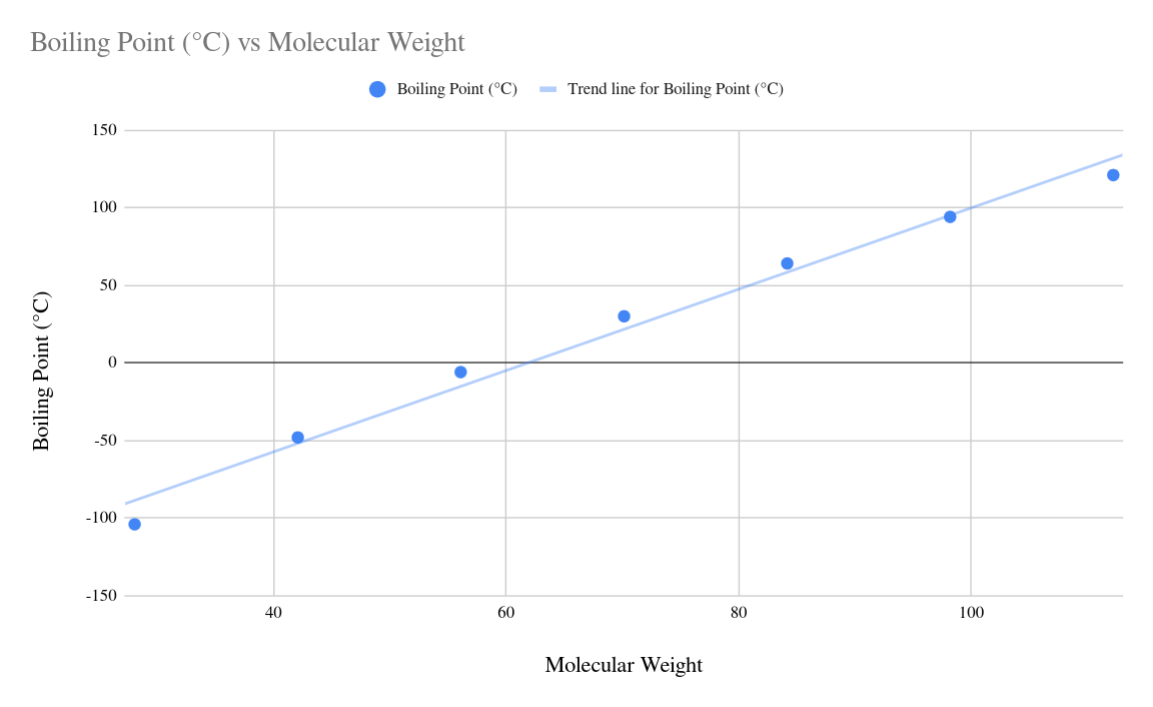
\includegraphics[width=15cm]{boiling_point_over_molecular_mass.png}
					\end{figure}

				\item \textit{Describe the trend shown on the graph.}

					There is a linear relationship between boiling point and molecular weight.

				\item \textit{Explain the trend in terms of intermolecular bonding.}

					Molecules with higher molecular masses have more atoms and can therefore induce more dispersion forces. More energy is required to break these bonds, hence molecules with higher molecular masses have higher boiling points than those of lower molecular mass.
			\end{enumerate}

		\item \textbf{Compound X has a boiling point of −6°C. Compound Y has a boiling point of 12°C. Compound Z has a boiling point of −55°C. All compounds are from the same homologous series.}

			\begin{enumerate}
				\item \textit{List the compounds in order of increasing molecular weight.}

					Compound Z, compound X, compound Y

				\item \textit{Explain your answer to part (a)}

					All 3 compounds are in the same homologous series and therefore share similar chemical formulae. Therefore, compounds with higher molecular weight will have higher boiling points
			\end{enumerate}

		\item \textbf{A compound has a relatively low boiling point, but is able to conduct electricity and is soluble in water. Is it likely to be a hydrocarbon? Justify your answer.}

			No. Hydrocarbons are non-polar and have no dipole charge and therefore cannot conduct electricity.

	\end{enumerate}

\newpage

\chapter*{Chapter 9 Review}

	\begin{enumerate}
		\item \textbf{Identify the functional group in each of the following compounds.}
			
			\begin{enumerate}
				\item Hydroxyl
				\item Carboxyl
				\item Amine
				\item Ester
				\item Carbonyl
				\item Carbonyl
				\item Amide
			\end{enumerate}

		\item \textbf{In general, in organic formulae an R group is often used. Explain what the R group represents.}

			The R group represents a general molecule.

		\item \textbf{Identify the functional group, draw its structure and give the general formula for alcohols, aldehydes, ketones and carboxylic acids.}
			
			\begin{table}[H]
				\centering
				\setstretch{1.25}
				\begin{tabular}{p{3cm}|p{3cm}|p{5cm}|p{3cm}}
					\textbf{Group}			& \textbf{Functional Group}		& \textbf{Structure}			& \textbf{General Formula}	\\ \hline
					Alcohol				& Hydroxyl				& \chemfig{-OH}				& \ce{C_{n}H_{2n+1}OH}		\\
									&					&					&				\\
					Aldehyde			& Carbonyl				& \chemfig{-C(=[2]O) - H}		& \ce{C_{n}H_{2n}O}		\\
									&					&					&				\\
					Ketone				& Carbonyl				& \chemfig{-C(-[2]O) -} 		& \ce{C_{n}H_{2n}O}		\\
									&					&					&				\\
					Carboxylic Acid			& Carbonyl				& \chemfig{-C(=[2]O) - OH} 		& \ce{C_{n}H_{2n}O2}		\\
				\end{tabular}
			\end{table}

		\item \textbf{Distinguish between an amine and amide in terms of structure and physical properties.}

			Amines are a functional group with a nitrogen atom and a lone pair in the form \ce{-NH2}. Amides form when the \ce{-OH} part of carboxylic acids is replaced by an amine functional group. Due to their \ce{N-H} bonds, both amines and amides have strong hydrogen bonding intermolecular forces. However, amides have a more polar functional group and therefore have higher boiling and melting points in comparison to that of amines.

		\item \textbf{For each of the following molecules, identify the homologous series it belongs to and write its correct IUPAC name.}
			\begin{enumerate}
				\item Alcohol, butan-2-ol
				\item Amide, N-methylethanamide
				\item Carboxylic acid, propanoic acid
				\item Amide, propanamide
				\item Ketone, 5-ethylhept-3-one
				\item Alcohol, 3-methylpentan-3-ol
			\end{enumerate}

		\item \textbf{Draw structural formulae for the following:}
			\begin{enumerate}
				\item 2-heptanol
					\subitem \chemfig{CH_3 - CH_2(-[2]OH) - CH_2 - CH_2 - CH_2 - CH_2 - CH_3} \\

				\item 4,5-dimethyl-2-hexanone
					\subitem \chemfig{CH_3 - C(=[2]O) - CH_2 - CH_2(-[2]CH_3) - CH_2(-[2]CH_3) - CH_3} \\

				\item 2-ethylbutanoic acid
					\subitem \chemfig{CH_3 - CH_2 - CH_2(-[2]CH_2(-[2]CH_3)) - C(=[1]O)(-[-1]OH)} \\

				\item 3-ethyl-1-hexanol
					\subitem \chemfig{CH_2(-[2]OH) - CH_2 - CH_2(-[6]CH_2(-[6]CH_3)) - CH_2 - CH_2 - CH_3} \\

				\item pentanamide
					\subitem \chemfig{C(-[4]NH_2)(=[2]O) - CH_2 - CH_2 - CH_2 - CH_3} \\

				\item 3-heptanamine
					\subitem \chemfig{CH_3 - CH_2 - CH(-[2]NH2) - CH_2 - CH_2 - CH_2 - CH_3} \\

				\item N-methylpropanamide
					\subitem \chemfig{C(-[4]N(-[-3]H)(-[3]CH_3))(=[2]O) - CH_2 - CH_2 - CH_3} \\

				\item 2-fluorobutanal
					\subitem \chemfig{CH(=[2]O) - CH(-[2]F) - CH_2 - CH_3} \\

				\item 3-methyl-2-butanone
					\subitem \chemfig{CH_3 - CH(=[2]O) - CH(-[2]CH_3) - CH_3} \\
			\end{enumerate}

		\item \textbf{Identify one alcohol, one aldehyde, and one carboxylic acid that have common names. Draw each molecule and give its correct IUPAC name.}
			
			Isopropyl alcohol (2-propanol)

				\begin{center}
					\chemfig{CH_3 - CH(-[2]OH) - CH_3}
				\end{center}

			Methanal (formaldehyde)

				\begin{center}
					\chemfig[angle increment = 30]{C(=[3]O)(-[-1]H)(-[-5]H)}
				\end{center}

			Acetic acid (ethanoic acid)

				\begin{center}
					\chemfig{CH_3 - C(=[1]O)(-[-1]H)}
				\end{center}

		\item \textbf{Draw structural formulae for the following and give the systematic names for:}
			\begin{enumerate}
				\item \textit{all isomers with molecular formula \ce{C3H8O}}
					
					\begin{table}[H]
						\centering
						\setstretch{1.25}
						\begin{tabular}{p{3cm}|p{9cm}}
							\textbf{Systematic Name}	& \textbf{Structural Formula}		\\ \hline
											&					\\
							Propan-1-ol			& \chemfig{CH_2(-[2]OH) - CH_2 - CH_3}	\\
											&					\\
							Propan-2-ol			& \chemfig{CH_3 - CH(-[2]OH) - CH_3}	\\
						\end{tabular}
					\end{table}

				\item \textit{carboxylic acids with molecular formula \ce{C4H8O}}

					\begin{table}[H]
						\centering
						\setstretch{1.25}
						\begin{tabular}{p{3cm}|p{9cm}}
							\textbf{Systematic Name}	& \textbf{Structural Formula}		\\ \hline
											&					\\
							Butanoic acid			& \chemfig{CH_3 - CH_2 - CH_2 - C(-[1]OH)(=[-1]O)}	\\
											&					\\
							2-methylpropanoic acid		& \chemfig{CH_3 - CH(-[-2]CH_3) - C(-[1]OH)(=[-1]O)}	\\
						\end{tabular}
					\end{table}
			\end{enumerate}

		\item \textbf{Compare the intermolecular forces and relative boiling points of the following classes of organic compounds.}

			\begin{enumerate}
				\item \textit Alkanes and alcohols
					\subitem Alkanes only have dispersion forces whereas alcohols have much stronger hydrogen bonds, as well as dispersion forces. Therefore, alcohols have higher boiling points than alkanes

				\item \textit Carboxylic acids and aldehydes
					\subitem Carboxylic acids have a hydrogen bond between an oxygen and hydrogen, creating strong intermolecular forces. Aldehydes do not have this bond and can only form dipole-dipole bonds. Hence carboxylic acids have higher boiling points

				\item \textit Alcohols and aldehydes
					\subitem Alcohols have hydrogen bonding whereas aldehydes don't, therefore alcohols have higher boiling points

				\item \textit Amines and amides
					\subitem Both amines and amides have strong intermolecular forces due to \ce{N-H} hydrogen bonds, however amides also have a double bonded oxygen that allows strong intermolecular forces to form, therefore amides have higher boiling points
			\end{enumerate}

		\item \textbf{Using examples from the alcohol, aldehyde, ketone, carboxylic acid, amine, or amide groups:}

			\begin{itemize}
				\item \textit{explain the difference between chain and positional isomers}
				\item \textit{explain the term ‘functional group isomer’.}
			\end{itemize}

			A chain isomer involves variations to the longest carbon chain of the molecule whereas a positional isomer is a rearrangement of the functional group.

			For example, pentan-2-ol and 2-methylbutan-2-ol represent chain isomers as they share the chemical formula \ce{C_5H_12O}

			\begin{table}[H]
				\centering
				\setstretch{1.25}
				\begin{tabular}{cc}
					\chemfig{CH_3 - CH(-[2]OH) - CH_2 - CH_2 - CH_3}	& \chemfig{CH_3 - C(-[2]CH_3)(-[-2]OH) - CH_2 - CH_3} \\
					pentan-2-ol						& 2-methylbutan-2-ol
				\end{tabular}
			\end{table}

			A positional isomer changes the location of the functional group, for example pentan-2-one and pentan-3-one, without changing the carbon structure.

			\begin{center}
				\chemname{\chemfig{CH_3 - CH(=[2]O) - CH_2 - CH_2 - CH_3}}{pentan-2-one}
				\qquad
				\chemname{\chemfig{CH_3 - CH_2 - CH(=[2]O) - CH_2 - CH_3}}{pentan-3-one}
			\end{center}

			Functional group isomers share the same molecular formula, however have a different functional group. For example, ketones and aldehydes have the same formulae, but vary depending on the location of the oxygen double bond.

			\begin{center}
				\chemname{\chemfig{CH_3(=[2]O) - CH - CH_3}}{propanal}
				\qquad
				\chemname{\chemfig{CH_3 - CH(=[2]O) - CH_3}}{propanone}
			\end{center}

		\item \textbf{Using the molecules 1-pentanol, 2-pentanol and 2-methyl-2-propanol, explain the difference between primary, secondary and tertiary alcohols.}
			
			Primary alcohols only have one carbon attached to the carbon that the \ce{-OH} group is attached to. In pentan-1-ol, the 1 carbon that the \ce{OH} group is only joined to the 2 carbon. Secondary alcohols have two carbons attached to the same carbon that the \ce{-OH} group is on. In pentan-2-ol, the hydroxyl group is attached to the second carbon, which itself is attached to the first and third hence making it a secondary alcohol. Tertiary alcohols have 3 carbons attached to the same carbon as the hydroxyl group and is the maximum number of carbons that can be attached.

			\begin{center}
				\chemname{\chemfig{CH_2(-[2]OH) - CH_2 - CH_2 - CH_2 - CH_3}}{pentan-1-ol}
			\end{center}
			\begin{center}
				\chemname{\chemfig{CH_3 - CH_(-[2]OH) - CH_2 - CH_2 - CH_3}}{pentan-2-ol}
			\end{center}
			\begin{center}
				\chemname{\chemfig{CH_3 - CH_(-[2]OH)(-[-2]CH_3) - CH_2 - CH_3}}{pentan-2-ol}
			\end{center}

		\item \textbf{Draw structures to describe the difference between primary, secondary, and tertiary:}

			\begin{itemize}
				\item amines
					\begin{table}[H]
						\centering
						\setstretch{1.25}
						\begin{tabular}{p{4cm}|p{8cm}}
							\textbf{Amine Type}	& \textbf{Diagram}		\\ \hline
										&				\\
							Primary			& \chemfig{C(-[2]H)(-[4]H)(-[-2]H) - C(-[2]H)(-[-2]H) - N(-[1]H)(-[-1]H)}	\\
										&				\\
							Secondary		& \chemfig{C(-[2]H)(-[4]H)(-[-2]H) - C(-[2]H)(-[-2]H) - N(-[1]H)(-[-1]C(-[0]H)(-[2]H)(-[-2]H))}	\\
										&				\\
							Secondary		& \chemfig{C(-[2]H)(-[4]H)(-[-2]H) - C(-[2]H)(-[-2]H) - N(-[1]C(-[0]H)(-[2]H)(-[-2]H))(-[-1]C(-[0]H)(-[2]H)(-[-2]H))}	\\
						\end{tabular}
					\end{table}

				\item amides
					\begin{table}[H]
						\centering
						\setstretch{1.25}
						\begin{tabular}{p{4cm}|p{8cm}}
							\textbf{Amide Type}	& \textbf{Diagram}		\\ \hline
										&				\\
							Primary			& \chemfig{CH_3 - CH_2 - C(=[2]O) - NH_2}	\\
										&				\\
							Secondary		& \chemfig{CH_3 - C(=[2]O) - N(-[1]H)(-[-1]CH_3)}	\\
										&				\\
							Tertiary		& \chemfig{CH_3 - C(=[2]O) - N(-[1]CH_3)(-[-1]CH_3)}
						\end{tabular}
					\end{table}
			\end{itemize}

		\item \textbf{Explain why molecules like glucose are soluble in water despite their high molecular weight.}

			Glucose has a large number of hydroxyl groups, creating many opportunities for hydrogen bonding with water.

		\item \textbf{Explain why the solubility of carboxylic acids and alcohols decreases as the length of their carbon chains increase.}
			
			As the length of the carbon chain of carboxylic acids and alcohols decrease, the effect of the dipole induced by the functional group is weakened across the whole molecule. This causes its solubility to decrease.

		\item \textbf{Explain why the boiling points of organic groups increase as the length of their carbon chains increase.}

			As the length of the carbon chain increases, there are more \ce{C-H} bonds that induce dispersion forces. This increases the strength of the bonding between molecules and increases the energy required to separate them.

		\item \textbf{Explain, using a specific example, how a dimer forms between two molecules. Use a diagram in your answer.}

			Under certain circumstances, a pure carboxylic acid can form a structure called a dimer. 

			\begin{figure}[H]
				\centering
				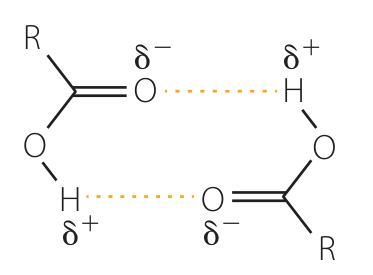
\includegraphics[width=10cm]{depth_study_dimer.png}
			\end{figure}

			In a dimer, the \ce{C=O} bond creates a hydrogen bond with the \ce{O-H} of another carboxylic acid. This arrangement increases the boiling point of the acid as there are now very strong intermolecular forces between molecules.

		\item \textbf{Carboxylic acids are weak acids. Describe one way their structure can be modified so their strength is increased. }
			
			A more electronegative halogen such as chlorine can be substituted in place of a hydrogen. This weakens the strength of the \ce{-OH} bond. The proton is more readily available to be donated, hence increases the strength of the acid.

		\item \textbf{Explain why citric acid is considered to be ‘more acidic’ than ethanoic acid.}

			Citric acid has three \ce{-OH} functional groups, and therefore more readily ionises in water in comparison to ethanoic acid with only one \ce{-OH} group. This means that citric acid is more acidic than ethanoic acid.

		\item \textbf{Explain why tertiary amines have lower boiling points and decreased solubility than similar molecular mass primary and secondary amines.}

			Primary and secondary amines have \ce{N-H} bonds that can form hydrogen bonds with other molecules such as water. Tertiary amines do not have the \ce{N-H} bond and therefore cannot form hydrogen bonds. This reduces the boiling point and solubility in comparison to primary and secondary amines.

		\item \textbf{Ethanol and water readily dissolve in each other, as do ethanol and hexane. However, water and hexane do not dissolve in each other.}

			\begin{enumerate}
				\item \textit{Draw structures of each molecule and explain whether it is polar or non-polar.}

					\begin{center}
						\chemname{\chemfig{H -[1]O -[-1]H}}{water - polar}
					\end{center}
					\begin{center}
						\chemname{\chemfig{C(-[2]H)(-[4]H)(-[-2]H) - C(-[2]H)(-[-2]H)(-[0]OH)}}{ethanol - polar}
					\end{center}
					\begin{center}
						\chemname{\chemfig{C(-[2]H)(-[4]H)(-[-2]H) - C(-[2]H)(-[-2]H) - C(-[2]H)(-[-2]H) - C(-[2]H)(-[-2]H) - C(-[2]H)(-[-2]H) - C(-[2]H)(-[0]H)(-[-2]H)}}{hexane - non-polar}
					\end{center}

				\item \textit{Explain why water and hexane do not dissolve in each other.}

					Molecules must share the same type of intermolecular forces in order for intermolecular bonding to occur. Water has hydrogen bonding whereas hexane only has dispersion forces and therefore they will not dissolve in each other.

				\item \textit{Explain, using diagrams showing intermolecular bonds, why ethanol can dissolve in both water and hexane.}

					The \ce{O-H} bonds in ethanol can form hydrogen bonds with water molecules, as well as dispersion force bonds with hexane.

				\item \textit{Considering your answer to part c, explain why ethanol is a widely used solvent in industry.}

					As stated, ethanol can form both hydrogen bonds through its hydroxyl group as well as dispersion forces. Hence, it can dissolve both polar and non-polar substances
			\end{enumerate}

		\item \textbf{Three compounds are known to be 1-propanol, ethanoic acid and propanone. Their boiling points (not in order) are 56°C, 118°C and 97°C. Match the correct boiling point to the compound, giving reasons for your answer.}

			\begin{center}
				\chemname{\chemfig{CH_3(-[2]OH) - CH_2 - CH_3}}{1-propanol}
			\end{center}
			\begin{center}
				\chemname{\chemfig{CH_3 - C(=[1]O)(-[-1] OH)}}{ethanoic acid}
			\end{center}
			\begin{center}
				\chemname{\chemfig{CH_3 - C(=[2]O) - CH_3}}{propanone}
			\end{center}

			Ethanoic acid has the highest boiling point of 118$\degree$C due to its hydroxyl group being able to form strong hydrogen bonds. Furthermore, it can form a dimer with itself, having very strong intermolecular forces.

			1-propanol will have a boiling point of 97$\degree$C as it can form hydrogen bonding through its hydroxyl group similar to carboxylic acids, however it lacks the polar \ce{C=O} bond that ethanoic acid has.

			Propanone has the lowest boiling point of 56$\degree$C as it only has dipole-dipole forces through its \ce{C=O} group.

		\item \textbf{Consider the table below showing the boiling points of various organic substances.}

			\begin{enumerate}
				\item \textit{Plot a graph of ‘number of carbons’ against boiling point for each of the three organic groups.}

					\begin{figure}[H]
						\centering
						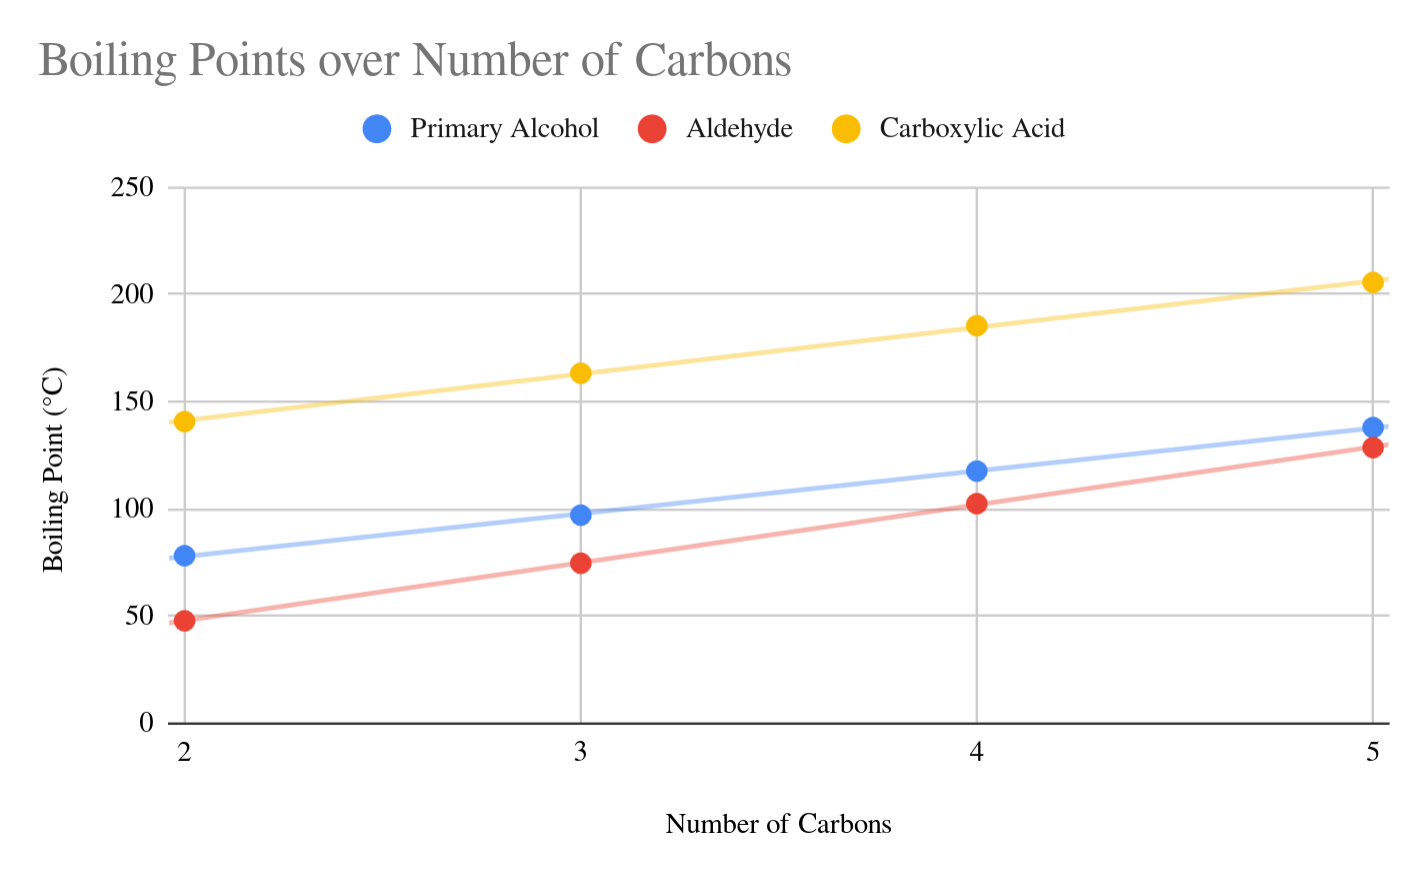
\includegraphics[width=15cm]{chapter_9_review_graph.png}
					\end{figure}

				\item \textit{Identify and explain two trends seen on the graph.}

					In all the hydrocarbons, as the length of the carbon chain increase so does the boiling point. This is due to increased dispersion forces that require more energy to break the intermolecular forces. As well as this, alcohols have higher boiling points in comparison to aldehydes with similar mass. This is due to the polar hydroxyl group forming a stronger bond with other molecules than that of the \ce{C=O} bond on aldehydes.

				\item \textit{Suggest a more valid way to compare these molecules than by "number of carbons".}

					The molecular weight of the molecules would be more appropriate way of comparing hydrocarbons. The number of carbons present does not accurately correspond to the molecules' sizes.
			\end{enumerate}

	\end{enumerate}

\newpage

\chapter*{Chapter 10 Review}

	\begin{enumerate}
		\item \textbf{Identify the key features contained within a SDS}

			An SDS outlines the potential risks and safety precautions necessary when using a specific chemical. The document will identify the compound, as well as other common names for the compound. It outlines the chemical and physical properties of the substance, as well as storage methods. Most importantly, it provides an extensive summary of risks associated with using the substance in reactions and states methods of reducing risk, as well as responses in case of exposure.

		\item \textbf{Explain the need for a document like a SDS to exist.}

			The document is a necessary safety measure to ensure that chemicals are used safely in both laboratories and industrial environments.
			
		\item \textbf{With reference to organic chemicals, explain the difference between the terms "volatile" and "flashpoint".}

			The volatility of an organic compound is the ability a substance to evaporate to form a vapour. Flashpoint refers to the lowest temperature at which a liquid can form an ignitable mixture in air.

		\item \textbf{From question 3, explain how knowledge of those properties allow for identification of risks when using organic chemicals.}

			Highly volatile chemicals pose risks for inhalation related poisoning and pose risks when used. As well as this, chemicals with low flashpoints are highly flammable, a property that should be accounted for when storing and using such chemicals.

		\item \textbf{Explain the difference between inhalation, ingestion, and absorption of chemicals}

			Inhalation occurs by breathing in a chemical and is the most common method of exposure since vapours are easily inhaled. Ingestion involves the chemical entering the body by being swallowed. This is usually done accidentally when chemicals are not properly handled and are present on hands or clothing. The absorption of chemicals is when they dissolve through the skin and enter the bloodstream.

		\item \textbf{Compare acute poisoning and chronic poisoning with reference to organic chemicals. You should include exposure methods and general symptoms in your answer.}

			Acute poisoning occurs immediately or soon after contact with a harmful chemical. Someone exposed may develop headaches, dizziness, poor coordination and may lose consciousness. Chronic poisoning occurs after repeated exposure and can develop over years or decades. Symptoms from chronic poisoning are usually more severe and may include chronic fatigue, physical weakness, and liver and kidney damage.
			
		\item \textbf{Identify key precautions you can take in your school investigations to minimise risks associated with using organic chemicals. Link each precaution to a specific risk you are trying to minimise.}

			At school, highly hazardous chemicals are avoided in experiments to reduce the chance of significant harm. Maintaining ventilation or using a fume cupboard clears vapours from an area and reduces the risk of chemical inhalation. As well as this, gloves and safety glasses are required to ensure that direct contact with chemicals is minimised.

		\item \textbf{What is the name given to the type of reaction where the following occurs?}

			\begin{enumerate}
				\item \textit{The addition of water to alkenes/alkynes}

					Hydration

				\item \textit{The addition of oxygen to hydrocarbons to produce energy}

					Combustion

				\item \textit{The addition of halogens to alkenes/alkynes}

					Halogenation

				\item \textit{The replacement of a hydrogen atom with a halogen atom in an alkane}

					Substitution
			\end{enumerate}

		\item \textbf{Write equations for:}

			\begin{enumerate}
				\item \textit{the hydration of pent-1-ene}

					\begin{center}
						\ce{\chemfig{CH_2 = CH - CH_2 - CH_2 - CH_3} + H2O ->[dilute H2SO4] \chemfig{CH_3 - CH(-[2]OH) - CH_2 - CH_2 - CH_3}}
					\end{center}

				\item \textit{the hydration of propyne}

					\begin{center}
						\ce{\chemfig{CH ~ C - CH_3} + H2O ->[dilute H2SO4] \chemfig{CH_3 = C(-[2]O) - CH_3}}
					\end{center}
			\end{enumerate}

		\item \textbf{Write equations for:}

			\begin{enumerate}
				\item \textit{the reaction of ethene with bromine}
					
					\begin{center}
						\ce{\chemfig{CH_2 = CH_2} + Br2 -> \chemfig{Br - CH_2 - CH_2 - Br}}
					\end{center}

				\item \textit{the reaction of ethane with chlorine under UV light}

					\begin{center}
						\ce{\chemfig{CH_3 - CH_3} + Cl2 ->[UV light] Cl - CH_2 - CH_2 - Cl}
					\end{center}

				\item \textit{the two step reaction of 1-butyne with chlorine}

					\begin{center}
						\ce{\chemfig{CH ~ C - CH_2 - CH_3} + Cl2 ->[UV light] \chemfig{CH(-[2]Cl) = C(-[2]Cl) - CH_2 - CH_3}}
					\end{center}
					\\
					\begin{center}
						\ce{\chemfig{CH(-[2]Cl) = C(-[2]Cl) - CH_2 - CH_3} + Cl2 ->[UV light] \chemfig{CH(-[2]Cl)(-[-2]Cl) - C(-[2]Cl)(-[-2]Cl)}}
					\end{center}

				\item \textit{the reaction of propene with hydrogen chloride}

					\begin{center}
						\ce{\chemfig{CH_2 = CH - CH_3} + HCl -> \chemfig{CH_3 - CH(-[2]Cl) - CH_3}}
					\end{center}
			\end{enumerate}

		\item \textbf{Write equations for:}
		
			\begin{enumerate}
				\item \textit{the complete combustion of 2-heptene}

					\begin{center}
						\ce{C7H14(l) + \frac{21}{2}O2(g) -> 7CO2(g) + 7H2O(l)}
					\end{center}

				\item \textit{the complete combustion of propyne}

					\begin{center}
						\ce{C3H4(l) + 4O2(g) -> 3CO2(g) + 2H2O(l)}
					\end{center}

				\item \textit{the combustion of 2-methylbutane}

					\begin{center}
						\ce{C4H10(l) + \frac{13}{2}O2(g) -> 4CO2(g) + 5H2O(l)}
					\end{center}
			\end{enumerate}

		\item \textbf{Write two equations to show different possible products in the incomplete combustion of butane.}

			\begin{center}
				\ce{C4H10(l) + \frac{9}{2}O2(g) -> 4CO(g) + 5H2O(l)}
			\end{center}
			\\
			\begin{center}
				\ce{C4H10(l) + \frac{5}{2}O2(g) -> 4C(g) + 5H2O(l)}
			\end{center}
			
		\item \textbf{Describe possible health issues with the production of carbon monoxide and soot in incomplete combustion.}

			Carbon monoxide is a colourless and odourless substance that is poisonous to humans, and therefore inhalation during an incomplete combustion is harmful. Soot particles can also be inhaled and restrict oxygen absorption into blood.

		\item \textbf{Describe the catalysts required for:}

			\begin{enumerate}
				\item \textit{hydrogenation of an alkene}

					The hydrogenation of an alkene requires a metal catalyst like palladium to increase the rate of reaction.

				\item \textit{production of margarine}

					Nickel metal catalyst

				\item \textit{conversion of an alkyne to an alkene}

					A Lindlar catalyst, usually palladium deposited onto calcium carbonate, prevents the hydrogenation reaction from further reacting the alkene into an alkane

				\item \textit{hydration of an alkene}

					Dilute \ce{H2SO4}

				\item \textit{hydration of an alkyne}

					Mercury(II) compound and \ce{H2SO4}
			\end{enumerate}

		\item \textbf{When water is added to 1-butene, two possible products are formed.}

			\begin{enumerate}
				\item \textit{Draw and name each possible product.}

					\begin{center}
						\chemname{\chemfig{CH_3 - CH(=[2]OH) - CH_2 - CH_3}}{butan-2-ol}
					\end{center}
					\\
					\begin{center}
						\chemname{\chemfig{CH_2(=[2]OH) - CH_2 - CH_2 - CH_3}}{butan-1-ol}
					\end{center}

				\item \textit{Explain which product is more likely to be formed and why.}

					Due to Markovnikov's rule, when an asymmetrical molecule is reacted with an asymmetrical hydrocarbon, the hydrogen from the reactant will join the carbon that has the most hydrogen atoms already attached. In the example of but-1-ene and water, the major product will be butan-2-ol.
			\end{enumerate}

		\item \textbf{In addition reactions, there are times when only one product can form, and times when multiple products can form.}

			\begin{enumerate}
				\item \textit{Using specific examples, explain how only one product can form.}

					When the reactant is symmetrical, then it can be evenly split between the carbon atoms with double or triple bonds. For example, the molecule \ce{Br2} will be evenly divided and one \ce{Br} atom will bond with each carbon.

				\item \textit{Using specific examples, explain how multiple products can form.}

					When an asymmetrical reactant such as water reacts with a hydrocarbon, it cannot split evenly. In the example of water, due to Markovnikov's rule, the carbon with more hydrogen atoms will gain additional hydrogen atoms, however both products are still possible.
			\end{enumerate}

		\item \textbf{Methane undergoes substitution reactions with chlorine under specific conditions.}
			\begin{enumerate}
				\item \textit{Identify what specific conditions are required for this reaction to occur.}
					
					Alkanes will only undergo a reaction if sufficient UV light is present.

				\item \textit{Explain how this knowledge can be used to distinguish alkanes and alkenes.}

					If bromine water is added to a sample of an alkene, it will decolourise, losing its orange-brown colour and becoming clear and colourless. If added to an alkane, no reaction will occur and it will remain orange brown.

				\item \textit{Write a series of equations to show the conversion of methane to tetrachloromethane}

					\begin{center}
						\ce{CH4 + Cl2 ->[UV light] ClCH3 + HCl} \\
						\ce{ClCH3 + Cl2 ->[UV light] Cl2CH2 + HCl} \\
						\ce{Cl2CH2 + Cl2 ->[UV light] Cl3CH1 + HCl} \\
						\ce{Cl3CH1 + Cl2 ->[UV light] Cl4C + HCl}
					\end{center}
			\end{enumerate}

		\item \textbf{You are given samples of heptane and 2-heptene}

			\begin{enumerate}
				\item \textit{Outline a method you could use to distinguish between the two samples. Include all chemicals used and what results you would expect.}

					Bromine water can be added to both samples. The heptane sample will maintain the brown-orange colour of the bromine water whereas the 2-heptene sample will become clear and colourless as the bromine reacts with the alkene.


				\item \textit{Identify one significant risk with the method you outlined, and how you would minimise its effects.}

					Bromine water has a harmful vapour that can cause illness if inhaled. Proper ventilation or a fume cupboard is required to use the above method.

				\item \textit{Write equations for any reactions that occurred}

					\begin{center}
						\ce{C7H14 + Br2 -> C7Br2H14}
					\end{center}
			\end{enumerate}

		\item \textbf{Four bottles containing clear liquids were found on the laboratory shelf with no labels. The bottles are known to contain 1-hexene, pentane, water and ethanol. A series of tests were conducted on each sample and the results are shown below.}

			\begin{enumerate}
				\item \textit{Using the information from the table, identify which bottle contained which chemical. Explain your answer.}

					Water is not flammable, and hence bottle A contains water. Ethanol is an alcohol and is soluble in water due to its ability to hydrogen bond with water molecules and is flammable and is therefore stored in bottle D. Bottle B decolourises bromine with the absence of UV light and hence must be 1-hexene. By deduction, bottle C must contain pentane Bottle B decolourises bromine with the absence of UV light and hence must be 1-hexene. By deduction, bottle C must contain pentane.

				\item \textit{Write equations for any reactions that occurred}

					Combustion of ethanol: \ce{C2H5OH(l) + \frac{7}{2}O2(g) -> 2CO2(g) + 3H2O(l)}

					Combustion of 1-hexene: \ce{C6H12(l) + 9O2(g) -> 6CO2(g) + 6H2O(l)}

					Combustion of pentane: \ce{C5H12(l) + 8O2(g) -> 5CO2(g) + 6H2O(l)}

					Bromine and 1-hexene: \ce{C6H12(l) + Br2(l) -> C6Br2H12(l)}

			\end{enumerate}

	\end{enumerate}

\newpage

\chapter*{Chapter 11 Review}

	\begin{enumerate}
		\item \textbf{Write equations to show:}

			\begin{enumerate}
				\item \textit{the dehydration of 1-propanol}

					\begin{center}
						\ce{\chemfig{CH_2(-[2]OH) - CH_2 - CH_3} ->[H+] \chemfig{CH_2 = CH - CH_3} + H2O}
					\end{center}

				\item \textit{the dehydration of 3-methyl-1-pentanol}

					\begin{center}
						\ce{\chemfig{CH_2(-[2]OH) - CH_2 - CH(-[2]CH_3) - CH_2 - CH_3} ->[H+] \chemfig{CH_2 = CH_2 - CH(-[2]CH_3) - CH_2 - CH_3} + H2O}
					\end{center}

				\item \textit{the reaction of 2-butanol with hydrogen bromide}
					
					\begin{center}
						\ce{\chemfig{CH_3 - CH(-[2]OH) - CH_2 - CH_3} + HBr -> \chemfig{CH_3 - CH(-[2]Br) - CH_2 - CH_3} + H2O}
					\end{center}

				\item \textit{the reaction of 2-methyl-2-pentanol with hydrogen chloride}

					\begin{center}
						\ce{\chemfig{CH_3 - C(-[2]OH)(-[-2]CH_3) - CH_2 - CH_2 - CH_3} + HCl -> \chemfig{CH_3 + C(-[2]Cl)(-[-2]CH_3) - CH_2 - CH_2 - CH_3 + H2O}}
					\end{center}

				\item \textit{the reaction of 2-methyl-2-bromobutane with water}

					\begin{center}
						\ce{\chemfig{CH_3 - C(-[2]Br)(-[-2]CH_3) - CH_2 - CH_3} + H2O -> \chemfig{CH_3 - C(-[2]OH)(-[-2]CH_3) - CH_2 - CH_3} + HBr}
					\end{center}

				\item \textit{the reaction of 1-chloroethane with water.}

					\begin{center}
						\ce{\chemfig{CH_2(-[2]Cl) - CH_3} + H2O -> CH_2(-[2]OH) - CH_3 + HCl}
					\end{center}
			\end{enumerate}

		\item \textbf{Write organic structural equations (not full balanced equations) for the oxidation of:}

			\begin{enumerate}
				\item \textit{2-propanol}

					\begin{center}
						\ce{\chemfig{CH_3 - CH(-[2]OH) - CH_3} ->[Cr2O7^2-] \chemfig{CH_3 - C(=[2]O) - CH_3}}
					\end{center}

				\item \textit{1-butanol}
					
					\begin{center}
						\ce{\chemfig{CH_2(-[2]OH) - CH_2 - CH_2 - CH_3} ->[Cr2O7^2-] \chemfig{C(=[3]O)(-[-3]H) - CH_2 - CH_2 - CH_3} ->[Cr2O7^2-] \chemfig{C(=[3]O)(-[-3]OH) - CH_2 - CH_2 - CH_3}}
					\end{center}

				\item \textit{2-methyl-1-pentanol}

					\begin{center}
						\ce{\chemfig{CH_3 - CH_2 - CH_2 - CH(-[2]CH_3) - CH_2(-[2]OH)} ->[Cr2O7^2-] \chemfig{CH_3 - CH_2 - CH_2 - CH(-[2]CH_3) - CH(=[1]O)(-[-1]H)} ->[Cr1O7^2-] \chemfig{CH_3 - CH_2 - CH_2 - CH - CH(=[1]O)(-[-1]OH)}}
					\end{center}

				\item \textit{2-methyl-3-hexanol}

					\begin{center}
						\ce{\chemfig{CH_3 - CH_2 - CH_2 - CH(-[2]OH) - CH(-[2]CH_3) - CH_3} ->[Cr2O7^2-] \chemfig{CH_3 - CH_2 - CH_2 - C(=[2]O) - CH_2(-[2]CH_3) - CH_3}}
					\end{center}
			\end{enumerate}

		\item \textbf{Write redox half reactions to show the reduction of dichromate ions and permanganate ions. Explain how these reactions can be used to visually test for the presence of a primary alcohol.}

			\ce{MnO4-(aq) + 8H+(aq) + 5e- -> Mn^2+(aq) + 4H2O(l)}

			Colour change from purple to colourless.

			\ce{Cr2O7^2-(aq) + 14H+ + 6e- -> 2Cr^3+(aq) + 7H2O(l)}

			Colour change from orange to green

		\item \textbf{You are given a sample of 1-pentanol and a sample of 2-methyl-2-pentanol. Both are colourless liquids but the labels have been removed.}

			\begin{enumerate}
				\item \textit{Outline an experiment you could perform to distinguish between the two compounds.}

					1-pentanol is a primary alcohol and added permanganate ions would go from purpose to colourless. 2-methyl-2-pentanol would not experience this colour change.

				\item \textit{Describe the observations you would make}

					Colour change as mentioned above.

				\item \textit{Explain how these observations allow you to tell the two compounds apart.}

					When dichromate or permanganate ions are added, one would experience a colour change, the other would not.
			\end{enumerate}

		\item \textbf{Samples of 2-methyl-2-bromopropane and 1-chloropropane are added to water. Explain which compound will be more reactive.}

			2-methyl-2-bromopropane is a tertiary haloalkane and will therefore be more reactive than the primary 1-chloropropane.

		\item \textbf{Explain, using bond energies, why:}

			\begin{enumerate}
				\item \textit{haloalkanes are more reactive than alkanes}

					The carbon-halogen bond is much easier to break than a \ce{C-H} or \ce{C-C} bond because carbon-halogen bonds have much lower bond energies.

				\item \textit{fluoroalkanes are very difficult to react}

					Fluoroalkanes have a \ce{C-F} bond with a bond energy higher than that of a \ce{C-H} and \ce{C-C} bond.
			\end{enumerate}

	\end{enumerate}

\newpage

\chapter*{Chapter 12 Review}

	\begin{enumerate}

		\item \textbf{Name the following compounds}

			\begin{enumerate}
				\item Ethyl propanoate
				\item Propyl propanoate
				\item Methyl butanoate
			\end{enumerate}

		\item \textbf{Draw structural formulae and give systematic names for all carboxylic acids or esters with the molecular formula \ce{C3H6O2}.}

			\begin{center}
				\chemname{\chemfig{CH(=[1]O) -[-1]O - CH_2 - CH_3}}{ethyl methanoate}
			\end{center}

			\begin{center}
				\chemname{\chemfig{CH_3 - C(=[1]O) -[-1]O - CH_3}}{methyl ethanoate}
			\end{center}

			\begin{center}
				\chemname{\chemfig{CH_3 - CH_2 - C(=[1]O) -[-1]OH}}{propanoic acid}
			\end{center}

		\item \textbf{Identify what type of isomerism is displayed in equation 2.}

			The esters are chain isomers, the carboxylic acid is a functional group isomer.

		\item \textbf{Compare an ester and a carboxylic acid of similar molecular mass in terms of:}

			\begin{enumerate}
				\item \textit{boiling point}

					Carboxylic acids form strong \ce{C-H} bonds whereas esters can only form dipole-dipole bonds. Therefore esters have higher boiling points

				\item \textit{solubility in water.} Carboxylic acids can form hydrogen bonds with water whereas esters cannot making carboxylic acids more soluble in water
			\end{enumerate}

		\item \textbf{Compare the general structure and properties of organic and inorganic acids.}

			By definition, organic acids contain carbon atoms whereas inorganic acids do not. However, they share similar properties such as the fact they both have hydrogen atoms that are relatively easy to lose. All organic acids are weak, whereas inorganic acids can be strong or weak.

		\item \textbf{A solution of oxalic acid has a pH of 1.31. A solution of ethanoic acid with the same concentration has a pH of 2.88. Give reasons for this difference.}

			Oxalic acid can more readily donate electrons in comparison to ethanoic acid due to its two carboxylic acid functional groups.

		\item \textbf{Write reactions for the addition of the following.}

			\begin{enumerate}
				\item \textit{1-propanol to butanoic acid}

					\ce{\chemfig{CH_3CH_2CH_2OH} + \chemfig{CH_3CH_2CH_2C(=[1]O)(-[-1]OH)} ->[reflux] \chemfig{CH_3CH_2CH_2C(=[1]O) -[-1]O - CH_2CH_2CH_3} + H2O}

				\item \textit{1-butanol to methanoic acid}

					\ce{\chemfig{CH_2OHCH_2CH_2CH_3} + \chemfig{CH(=[1]O) -[-1]OH} ->[reflux] \chemfig{CH(=[1]O) -[-1]O - CH_2CH_2CH_2CH_3} + H2O}

				\item \textit{Lithium metal to butanoic acid}

					\ce{2CH3CH2CH2COOH(aq) + 2Li(s) <=> 2CH3CH2CH2COO^-(aq) + 2Li^+(aq) + H2(g)}

				\item \textit{Sodium hydroxide to methanoic acid}

					\ce{HCOOH(aq) + NaOH(aq) <=> HCOO^-(aq) + Na^+(aq) + H2O(l)}

				\item \textit{Sodium carbonate to 2-methylpentanoic acid}

					\ce{2CH3CH2(CH3)CH2CH2COOH(aq) + Na2CO3(aq) <=> 2CH3CH2(CH3)CH2CH2COO^-(aq) + 2Na^+(aq) + H2O(l) + CO2(g)}

				\item \textit{Hydrochloric acid to propanamine}

					\ce{CH3CH2CH2NH2(aq) + HCl(aq) <=> CH3CH2CH2NH3^+(aq) + Cl^-(aq)}
			\end{enumerate}

		\item \textbf{Outline a method for the chemical test that could be used to distinguish between the following pairs of compounds}

			\begin{enumerate}
				\item \textit{1-butanol and butanoic acid}

					Butanoic acid will react with sodium carbonate solution to form gas bubbles whereas 1-butanol will not.

				\item \textit{2-propanol and 2-methyl-2-propanol}

					2-propanol will turn acidified dichromate ions green

				\item \textit{Heptane and 2-heptene}

					Heptene will react in bromine water, creating a colourless solution whereas heptane will remain brown.

				\item \textit{Ehtyne and ethyl ethanoate}

					Ethyl ethanoate will decolourise bromine water where ethyne will not.
			\end{enumerate}

		\item \textbf{Flow charts represent chemical processes in a different form from text and equations. Identify:}

			\begin{enumerate}
				\item \textit{two benefits of using flow charts over other representations}

					Flow charts provide a simple visual method of looking at reactions between chemicals and can be followed as a line of processes

				\item \textit{two limitations of using flow charts over other representations.}

					Flow charts do not show the equations for reactions occurring and are usually generalised.
			\end{enumerate}

		\item \textbf{Choose an appropriate alkane/alkene and describe the steps you would take to prepare:}

			\begin{enumerate}
				\item \textit{hexanoic acid}

					Using \ce{H2SO4} as a catalyst, hex-1-ene can be reacted with water to form hexan-1-ol. This hexan-1-ol can be oxidised with acidified dichromate ions and concentrated sulphuric acid to produce hexanal that further oxidises into hexanoic acid.

				\item \textit{butanal.}

					But-1-ene is combined with water with a dilute sulphuric acid catalyst to form butan-1-ol. This can then be oxidised with acidified dichromate ions and a concentrated sulphuric acid catalyst to produce butanal.
			\end{enumerate}

		\item \textbf{Explain the need for the following steps in ester production and purification}

			\begin{enumerate}
				\item \textit{Reflux for 30 minutes}

					Reflux allows volatile components to evaporate and condense back into liquids and maximise the yield of ester produced.

				\item \textit{Washing the reaction mixture with water in a separating funnel}

					Washing the reaction mixture in water allows the carboxylic acids and alcohols to dissolve, leaving a more pure ester.

				\item \textit{Addition of sodium carbonate to the reaction mixture.}

					Dissolves the long chain carboxylic acids that do not dissolve in water.
			\end{enumerate}

		\item \textbf{Identify two significant risks when preparing and purifying esters. Describe precautions you should take to minimise these risks}

			Organic chemicals can be flammable and a heating mantle should be used rather than a Bunsen burner. An open flame should not be exposed to any gases why producing esters. As well as this, gas build up can occur when purifying an ester with sodium carbonate. The separating funnel should not be stoppered until all gas forms and escapes.

	\end{enumerate}

\newpage

\chapter*{Chapter 15 Review}

	\begin{enumerate}
		\item \textbf{What chemical tests would you use to distinguish between the following pairs of compounds?}

			\begin{enumerate}
				\item \textit{1-butanol and butanoic acid}

					Butanoic acid will react with sodium carbonate solution and begin to bubble whereas butan-1-ol will not.

				\item \textit{2-propanol and propane}

					Permanganate will reaction with propan-2-ol and oxidise it into propan-2-one.

				\item \textit{Octane and 2-pentene}

					Pent-2-ene will react with bromine water and go from brown to clear and colourless. Octane will not react.
			\end{enumerate}

		\item \textbf{Write equations for the following reactions and name the products.}

			\begin{enumerate}
				\item \textit{2-hexanol and sodium metal}

					\ce{2CH3CH2CH2CH2OHCH3(l) + 2Na(s) -> 2CH3CH2CH2CH2O^- Na^+(aq) + H2(g)}

					Products: sodium hexoxide and hydrogen gas

				\item \textit{Pentanoic acid and sodium carbonate}

					\ce{CH3CH2CH2CH2COOH(aq) + Na2CO3(aq) -> 2CH3CH2CH2CH2COO^- Na^+(aq) + CO2(g) + H2O(l)}

					Products: sodium pentanoate, carbon dioxide, water

				\item \textit{Bromine water and ethene}

					\ce{Br2(aq) + CH2=CH2(l) -> CH2BrCH2Br(l)}

					Products: 1,2-dibromoethane
			\end{enumerate}

		\item \textbf{Compare the use of instrumental analysis techniques with chemical testing, giving advantages and disadvantages of each.}

			Chemical testing is cheaper and provides a quick but less detailed analysis of a substance. It cannot show some properties such as molecular structure. As well as this, the sample is changed during the process of testing. Instrumental techniques require much more precision and highly specialised and expensive equipment. Due to this, they can generally only be performed in laboratories.

		\item \textbf{Which instrumental technique would be the easiest to use to distinguish carbohydrates, esters, carboxylic acids, and amino acids?}

			IR spectroscopy should be used as it shows different functional groups.

		\item \textbf{What information is given in a 1H and 13C NMR spectrum? Why is NMR spectroscopy such a valuable technique for determining the structure of proteins and larger molecules?}

			In H-NMR, the number of different hydrogen environments is given. High resolution NMR can also provide the number of hydrogen atoms on adjacent carbon atoms. Carbon NMR shows the different environments of carbon.

		\item \textbf{Which technique is the best for determining the molar mass of a compound?}

			Mass spectroscopy

		\item \textbf{Why is the molar mass for an element given on the period table not a whole number?}

			The mass given is the average of the isotopes present for the element.

		\item \textbf{What characteristic peaks would you expect in a mass spectrum of a chloroalkane?}

			A peak would be expected at 35 due to the molar mass of chlorine present in the chloroalkane.

		\item \textbf{A chemist had three liquids: ethanol, butanoic acid and 3-heptene, but did not know which was which so called them P, Q and R. When drops of bromine solution were added to samples of each liquid, Q decolourised the bromine but P and R did not. When drops of sodium carbonate solution were added to fresh, dry samples of the three liquids, R produced bubbles of colourless gas but P and Q did not. When a piece of sodium metal was added to fresh samples of the three liquids P and R produced bubbles of gas but Q did not.}

			P decolourised bromine and reacted with sodium metal but not sodium carbonate, and therefore must be ethanol.

			Q only decolourised bromine and therefore must be hept-3-yne.

			R must therefore be butanoic acid.

		\item \textbf{A compound was formed from the reaction of an alkene and HCl. The compound was 46\% carbon and 9\% hydrogen.}

			\begin{enumerate}
				\item \textit{Determine the emperical formula for the compound}

					\ce{C3H7Cl}

				\item \textit{Examine the mass spectrum (Figure 15.32) of the compound. What is the molecular formula for the compound?}

					Parent peak is 78, therefore the molecular formula is \ce{C3H7Cl}

				\item \textit{Why is the parent peak not the peak with the largest m/z value in this case?}

					Chlorine has the isotopes of 35 and 37. 35 is more abundant and is therefore used to determine the parent peak.

				\item \textit{Draw the possible isomers for the compound}

					\begin{center}
						\chemfig{CH_3 - CH_2 - CH_2 - Cl}
					\end{center}
					\begin{center}
						\chemfig{CH_3 - CH(-[2]Cl) - CH_3}
					\end{center}

				\item \textit{Account for peaks at 43, 63, and 65.}

					The peak at 43 would be due to the loss of chlorine. The peak at 63 would be the loss of a methyl group. The peak at 65 would be due to the loss of a methyl group from a parent peak of chlorine 37 isotopes.

				\item \textit{Use the mass spectrum to decide which one is the most likely isomer.}

					The most likely isomer is the second one.
			\end{enumerate}

		\item \textbf{In court, criminals may claim that they were producing a perfume and not an illicit drug. How would infrared analysis help forensic scientists discredit the criminal? Would it be an advantage to take samples from the clandestine laboratory over time?}

			IR spectroscopy can be used to identify the functional groups present.

		\item \textbf{NMR and mass spectra can be used to determine the structures of molecules. How do these techniques differ in this task? Is just one of these sufficient to determine the structure?}

			Mass spectroscopy provides information about the parent mass of a molecule, as well as the ways it can be broken apart. NMR gives information about the different hydrogen or carbon environments of a molecule, providing more about its structure. Complex molecules require both methods to be used.

		\item \textbf{How many peaks would be expected in a 1H NMR spectrum for propanone (CH3COCH3)?}

			Only 1 because it is symmetrical.

		\item 
			\begin{enumerate}
				\item \textit{How could 13C NMR spectroscopy be used to distinguish between 1-nitropropane and 2-nitropropane?}

					In 1-nitropropane, there would be three carbon environments whereas in 2-nitropropane there would only be two.

				\item \textit{Would the 1H NMR provide more information? If so what information would it provide?}

					H-NMR would provide the ratio of hydrogen on each carbon atom.
			\end{enumerate}

		\item \textbf{What differences would you expect in a mass spectrum of 1-propanol and 2-propanol?}

			Alcohols usually fragment at the \ce{C-COH} bond. 1-propanol would peak at 29 and 21, whereas 2-propanol would peak at 15 and 45.

		\item \textbf{X is an organic compound composed of carbon, hydrogen and oxygen. It contains 48.63\% carbon and 8.18\% hydrogen by mass.}

			\begin{enumerate}
				\item \textit{Calculate the empirical formula of X.}

					\ce{C3H6O2}

				\item \textit{The mass spectrum for X is shown in Figure 15.33.}

					\begin{enumerate}
						\item Deduce, giving a reason, the molecular formula of X.

							The parent peak is at 74, therefore the molecule has a mass of 74. Hence, the molecular formula is \ce{C3H6O2}

						\item Identify the formulae of the fragment ions with m/z values of 45 and 29.

							At 45, the fragment ion would be due to \ce{COOH+}. At 29, it could be due to either \ce{CH3CH2+} or \ce{CHO+}
					\end{enumerate}

				\item \textit{The infrared spectrum of X is shown in Figure 15.34.}

					\begin{enumerate}
						\item Explain why X is not a carboxylic acid.

							There is no broad peak around 2500-3100 that indicates a hydroxyl group.

						\item Identify, giving reasons, three bonds that are present in X.

							From left to right, the three peaks on the IR spectrum indicate \ce{C-H}, \ce{C-C}, and \ce{C=O} bonds.
					\end{enumerate}

				\item \textit{Deduce the most likely structural formula of X based on your answers to parts b and c. State the name of X and give one use of compounds belonging to this homologous series.}

					The most likely structural formula is ethyl methanoate.

					\begin{center}
						\chemfig{CH(=[1]O) -[-1]O - CH_2 - CH_3}
					\end{center}

				\item \textit{State and explain the number of peaks compound X will show in its low-resolution 1H NMR spectrum.}

					There are three hydrogen environments and therefore 3 peaks.

				\item \textit{State the names of two compounds that could react together to produce X. Identify the type of reaction and give an equation for the reaction.}

					Ethanol and methanoic acid can be reacted in esterification to form ethyl methanoate.
			\end{enumerate}

		\item \textbf{Assign the peaks for the mass spectrum in the figure below. Is the compound tested 1,2-ethanediol? How many peaks would you expect in the 1H NMR spectrum and the 13C NMR spectrum?}

			The parent peak at 62 is consistent with the molar mass of 1,2-ethanediol. As well as this, the fragment \ce{CH2OH+} is also consistent.

		\item \textbf{The figure below is the 1H NMR spectrum of a compound with molecular formula \ce{C2H4Br2}. Use the information in the spectrum to determine the structure of the compound.}

			\begin{center}
				\chemfig{C(-[2]H)(-[-2]H)(-[4]H) - C(-[2]H)(-[-2]Br)(-Br)}
			\end{center}

		\item \textbf{Compare the following 13C NMR, infrared and mass spectra. Assign each to ethanol, ethanoic acid or ethyl ethanoate. Justify your choices.}

			\begin{enumerate}
				\item Ethanol
				\item Ethanoic acid
				\item Ethyl ethanoate
				\item Ethanol
				\item Ethyl ethanoate
				\item Ethanoic acid
			\end{enumerate}
	\end{enumerate}

\newpage

\section*{Practical Investigation 15.1}

	\textbf{Aim}: To identify an unknown hydrocarbon.

	\subsubsection{Materials}

		\begin{itemize}
			\item Blue litmus paper
			\item Calcium carbonate solution
			\item Bromine water
			\item Calcium chloride
			\item Sodium
			\item Acidified potassium permanganate
		\end{itemize}
	
	
	\subsubsection{Method}
		
		\begin{enumerate}
			\item Use blue litmus paper to test acidity. If the paper turns red then the solution is acidic. Furthermore, add calcium carbonate solution. If bubbles form, then it is a carboxylic acid.
			\item Apply bromine water to the solution. If it remains brown-orange, then it does not contain any double or triple bonds. If the solution becomes clear and colourless, then the hydrocarbon has multiple bonds.
			\item Add granules of calcium chloride to remove water, then add sodium. If hydrogen gas forms, then it is an alcohol.
		\end{enumerate}

\newpage

\section*{Practical Investigation 15.2}

	\textbf{Aim}: To identify structures from infrared and mass spectra data provided

	\subsubsection{Method}
	
		\begin{enumerate}
			\item Examine the six molecules A–F and spectra 1–6.
			\item Match the spectra to the organic molecules. (Hint: Calculate the molar mass.)
			\item Look for possible common fragments.
			\item Look for key functional groups in the infrared spectra.
		\end{enumerate}

	\subsubsection{Results}
	
		\begin{itemize}
			\item Spectra 1 - F
			\item Spectra 2 - C
			\item Spectra 3 - A
			\item Spectra 4 - E
			\item Spectra 5 - D
			\item Spectra 6 - B
		\end{itemize}

\end{document}

